 \chapter{引言}
\label{cha:intro}

\section{研究背景与研究意义}
\label{sec:background}
\subsection{新能源电力系统发展现状}
日益严峻的全球环境及气候变化挑战,使得大多数国家和地区聚焦于可再生能源的持续开发与高效利用。实现高比例的可再生能源电力供应已渐成共识
\cite{Obama-Science-17,Balance-Nature16,Chu-Nature-12}, 欧盟、美国、中国分别提出2050年实现100\%、80\% 及60\% 的可再生能源电力供应规划\cite{PS-Flexibility-Plan-LZX-16}。美国纽约州出台了于2030 年实现50\%可再生能源电量渗透的REV 2030 Goals 规划
\footnote{https://rev.ny.gov/rev-goals-2030/};2018年8月,美国加州出台了于2045年实现100\% 可再生能源电量渗透的SB100 法案\footnote{https://ca100.org/}。

在高比例可再生能源电力供给实践方面,部分国家和地区已取得初步成效。2016年, 葡萄牙实现了107小时的100\% 可再生能源电力供应\footnote{https://reneweconomy.com.au/portugal-reaches-100-renewables-ends-fossil-fuel-subsidies-32820/}。 青海电网于2017年6月在国内率先实现了“绿电7 日”运行,以水、风、光等可再生能源供电,期间水电供电72.3\%,新能源供电27.7\%,在100\% 可再生能源电力系统方面做了初步探索。2018年6月,青海电网进一步实现了“绿电9 日”运行,期间水电供电79.36\%,新能源供电20.74\%\footnote{http://www.nea.gov.cn/2018-06/27/c$\_$137284329.htm}。 诚然,当前的新能源电力系统仅能实现较短时间的高比例可再生能源电力供应,如何实现可持续的高比例可再生能源电力供应值得探讨。

\begin{figure}[H] % use float package if you want it here
  \centering
  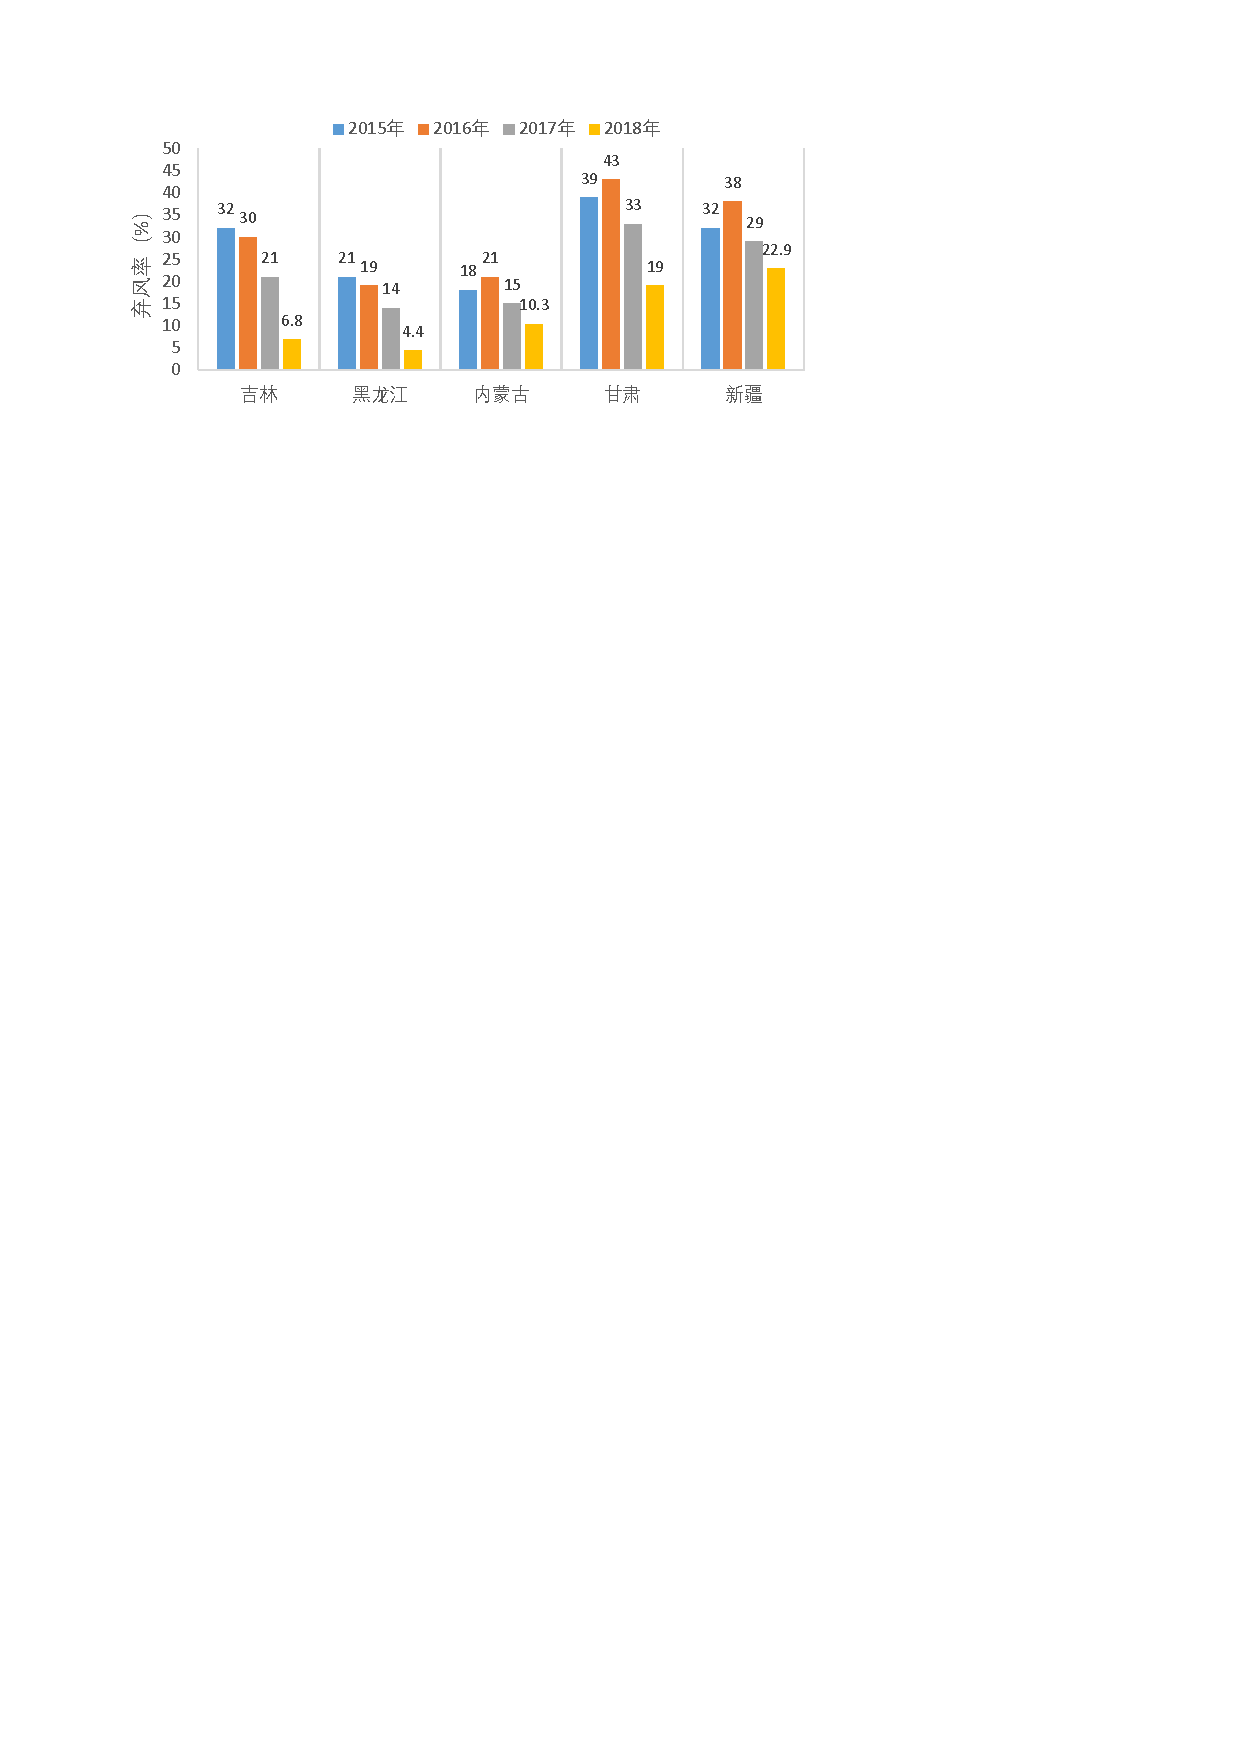
\includegraphics[scale=0.95]{figures/Chap1-1-Wind-Curtailment-Province.pdf}
  \caption{典型省份弃风数据(2015-2018)}
  \label{fig:Wind-Curtailment-Province}
\end{figure}

近年来,高比例可再生能源电力系统的发展遇到一定挑战,主要表现为新能源电力并网导致的高比例消纳难题与负电价现象。受限于电网设备利用率偏低、能源结构中煤炭占比高等因素~\cite{Renewable-Consum-17},我国西北、东北等可再生能源装机容量渗透水平较高地区,弃风问题较为严重。2016 年,吉林、黑龙江弃风分别达30\%与19\%, 内蒙古弃风达21\%, 甘肃与新疆弃风分别达43\%与38\%,如图~\ref{fig:Wind-Curtailment-Province}~所示\footnote{数据整理自国家能源局, http://www.nea.gov.cn}。通过可再生能源优先发电、可再生能源电力参与市场化交易、可再生能源电力配额制、省间跨区协调、负荷电气化等措施的相继实施\footnote{国家能源局《解决弃水弃风弃光问题实施方案》, 国家电网《促进新能源发展白皮书》(2018)。},2017 年吉林、黑龙江弃风分别降为21\%与14\%, 内蒙古弃风降为15\%, 甘肃与新疆分别降为33\% 与29\%;2018年吉林、黑龙江弃风分别降至6.8\% 与4.4\%, 内蒙古降至10.3\%, 甘肃与新疆电网弃风分别降至19\%与22.9\%。尽管弃风问题有了一定程度的改善,但受限于新能源电力系统本身灵活性资源的缺乏,系统能继续接纳的可再生能源电力比例受限,维持较低的弃风水平的前提是风电装机容量的缓慢增长,如图~\ref{fig:Wind-Installment-Capacity}~所示\footnote{图中数据整理自国家能源局, http://www.nea.gov.cn}。

\begin{figure}[H] % use float package if you want it here
  \centering
  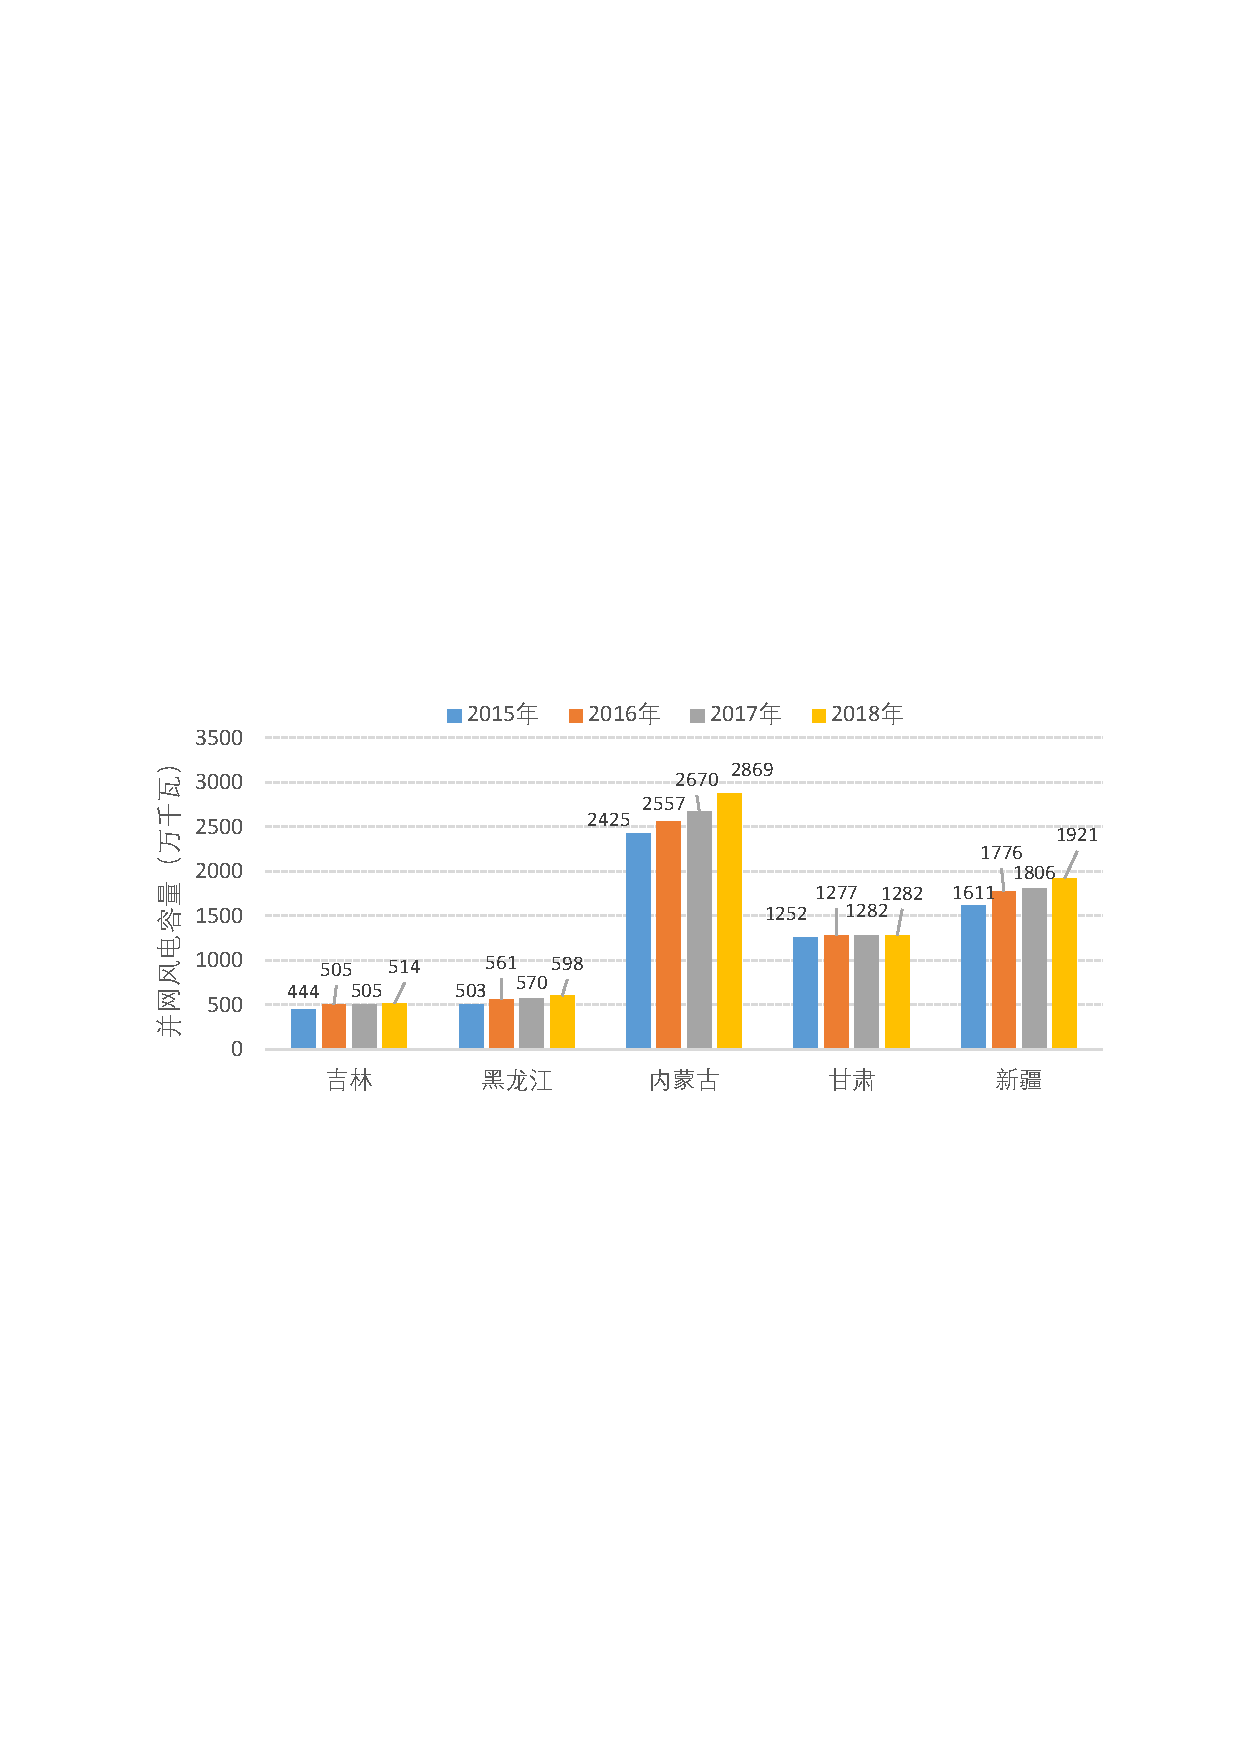
\includegraphics[scale=0.75]{figures/Chap1-1-Wind-Installment-Capacity.pdf}
  \caption{典型省份风电并网装机容量(2015-2018)}
  \label{fig:Wind-Installment-Capacity}
\end{figure}

受限于新能源电力的波动性,美国、德国等国家出现了较为频繁的负电价现象, 且有愈演愈烈之势\cite{Neg-Price-US-Evidence,Neg-Price-German-13}。以可再生能源资源丰富的美国加州CAISO 电力批发市场为例,SP-15节点2014年负电价小时数占比为5.03\%, 2015年升为5.40\%, 2016 年升至8.33\%\cite{Neg-Price-US-Evidence}。 同时,PJM、ERCOT、ISO-NE、NYISO等电力市场负电价占比也在(持续)增长,如表~\ref{tab:neg-price-US}所示。辨识影响可再生能源电力发展的关键因素,是实现可持续的高比例可再生能源电力供应的前提。

\begin{table}[htb]
  \centering
  \begin{minipage}[t]{0.8\linewidth} % 如果想在表格中使用脚注,minipage是个不错的办法
  \caption{美国电力市场典型节点负电价小时数占比变化(2013-2016)
  \footnote{表中数据整理自文献\inlinecite{Neg-Price-US-Evidence}。}}
  \label{tab:neg-price-US}
    \begin{tabularx}{\linewidth}{cccccc}
      \toprule[1.5pt]
      {\heiti 年份} & {\heiti CAISO} & {\heiti ERCOT} &  {\heiti NYISO} & {\heiti PJM} & {\heiti ISO-NE} \\\midrule[1pt]
      2013 &	2.26\%	& 0.29\%  & 1.37\%	& 2.41\%  & 0.00\%  \\
      2014 &	5.03\%	& 0.67\%  & 2.13\%	& 5.24\%  & 0.76\%  \\
      2015 &    5.40\%	& 3.79\%  & 8.56\%	& 11.00\% & 1.64\%  \\
      2016 &    8.33\%	& 3.94\%  & 6.54\%	& 4.01\%  & 2.77\%  \\
      电价节点 &	SP-15 & 	West & 	ZoneD-North &	Byron &	Maine\\
      \bottomrule[1.5pt]
    \end{tabularx}
  \end{minipage}
\end{table}

事实上,中国三北地区存在的新能源消纳难题与美国、德国等出现的负电价现象主要受新能源电力系统中电源、电网及负荷三侧的因素综合影响,具体表现在:1)受风/光资源与风/光功率间的瞬时强耦合关系,源侧并网的新能源电力具有较强的波动性与随机性;2)网侧的灵活调节容量、输送通道容量等因素的限制,难以为源侧注入的不确定性提供充足的灵活性资源~\cite{Renewable-Consum-17};3)荷侧聚焦于电能形式的消纳模式难以有效发挥终端热电协同调控对新能源电力系统灵活性资源的支撑作用~\cite{,EH-FREEDM-11,Smart-Grid-Energy-Internet-14,IES-Review}。

\subsection{压缩空气储能及支撑政策}
大规模储能(储电、储热)技术是平滑新能源出力波动性、提高输电通道平均利用率、提供灵活调峰容量及实现新能源电力热电协同调控的主要措施之一~\cite{Balance-Nature16,ESS-Engineering-15,TES-CSP-12}。为支撑2050 年可再生能源发展规划,美国、欧洲、中国等市场的储能容量总需求达450GW ~\cite{IEA-Report-14}。 目前已商业化的大规模物理储能技术主要包括抽水蓄能和压缩空气储能(Compressed Air Energy Storage, CAES)\footnote{本文设定CAES指代压缩空气储能技术,不涉及其具体实现方案,如等温、绝热及非绝热等。},前者约占全球~141GW(2017年)储能容量的99\%,但因建址条件及潜在生态环境等因素,发展已渐趋平缓~\cite{IEA-Report-14}。 近二十年来,CAES 因容量大、寿命长、响应速度快等优点得到了国内外多个大型企业及研究机构的关注,欧、美、日、中、加等也纷纷部署了CAES 技术发展路线~\cite{CAES-Review-16-Polygeneration,CAES-Review-09,CAES-Review-16-Rui,CAES-Review-17}。

先进绝热压缩空气储能(Advanced Adiabatic Compressed Air Energy Storage, AA-CAES)是一种通过空气压缩热能的回收再利用摒弃燃料补燃的新型CAES技术形式~\cite{ACAES-Green-12}, 其工作原理如图~\ref{fig:AA-CAES-principle-abs}~所示。压缩储能时, AA-CAES 利用弃风(光)、低谷电等电能或风能等机械能驱动压缩机,经绝热压缩(压缩系统)回收压缩热,解耦存储空气压力势能(储气库)和压缩热能(蓄热系统);膨胀释能时,通过绝热膨胀(透平系统\footnote{文献中透平系统亦称为膨胀系统,本文对二者不加区分。})利用压缩热能,实现空气压力势能和压缩热能的耦合释能。

与电池储能、抽水蓄能等储能技术不同,AA-CAES除了能提供常规储能具有的能量搬移与容量备用方面的灵活性~\cite{CAES-Baseload-Review-12,CAES-Reserve-11}外,还能为新能源电力系统注入供能灵活性及接口灵活性,主要表现在:1)蓄热系统(换热器与储热罐)的存在使AA-CAES 具备了潜在的热电联供与热电联储能力,其既可配置于电力系统电能单能流应用场景,也可应用于区域热电综合能源系统热电多能流场景,具有一定的供能灵活性~\cite{CAES-Review-18-Rui-operation,CAES-Review-16-Polygeneration}; 2)AA-CAES可以风能等机械能作为输入接口直接驱动,亦可以输出机械能直接驱动动力机械等,具有良好的接口灵活性,有望实现风-储集成设计,进而从源头上改善风电功率的波动性。

\begin{figure}[H] % use float package if you want it here
  \centering
  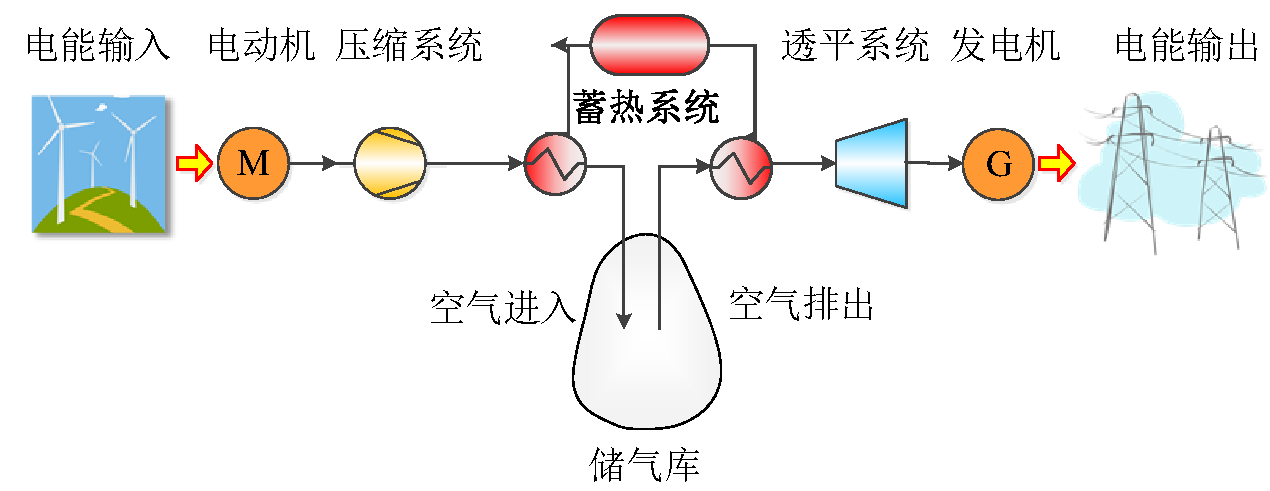
\includegraphics[scale=0.60]{figures/Chap1-1-AA-CAES-Principle-Abs.pdf}
  \caption{AA-CAES工作原理示意图}
  \label{fig:AA-CAES-principle-abs}
\end{figure}

AA-CAES具有的常规、供能、接口等三类灵活性可为从源—网—荷三侧支撑可持续的高比例可再生能源电力供应提供新的思路,也因此成为目前CAES 领域的主流技术~\cite{AA-CAES-04,AA-CAES-07},备受我国能源电力部门的青睐。2016年6月,CAES技术被纳入《中国制造2025—能源装备》计划;与此同时相关储能支撑政策不断出台,加快了储能示范项目的商业化进程~\cite{ESS-CESA-16,ESS-CIAPS-16}。《关于推进电能替代的指导意见》
\footnote{http://www.ndrc.gov.cn/gzdt/201605/t20160524$\_$804439.html} 鼓励拉大峰谷价差,以提高储能经济性;《关于促进电储能参与“三北”地区电力辅助服务补偿(市场)机制试点工作的通知》
\footnote{http://zfxxgk.nea.gov.cn/auto92/201606/t20160617$\_$2267.htm} 鼓励储能设施参与辅助服务市场,进一步创造储能收益源;《关于促进储能技术与产业发展的指导意见》
\footnote{http://www.nea.gov.cn/2017-10/11/c$\_$136672015.htm},描绘了储能10 年发展蓝图——“十三五”期间进入商业化初期,“十四五”期间实现规模化发展;《关于进一步深化电力体制改革的若干意见(中发[2015]9号)文》
\footnote{http://www.nea.gov.cn/2015-11/30/c$\_$134867851.htm} 及系列配套文件为建立健全辅助服务市场及储能参与辅助服务提供了市场条件。

\subsection{研究意义}
随着压缩机、换热器、储气库、储热及透平膨胀机\footnote{文献中透平膨胀机存在多种名称,包括膨胀机、空气透平及空气透平膨胀机等,本文不加以区分。}等关键技术的突破~\cite{CAES-Review-17-Rui-salt,TES-CSP-review-13},以及国内外多项示范工程的逐步落实与有序推进,AA-CAES将从平滑新能源电力的波动(源侧)、提供灵活调节容量(网侧)及支撑热电协同调控(荷侧)等方面促进可再生能源电力的可持续高比例接纳。

在电能单能流应用场景下,AA-CAES 可配置在风电光伏场站侧,形成风光/储混合系统承担系统基荷,缓解输电线路阻塞、提高输电线路载荷率、延缓输配线扩容;亦可部署于负荷侧支撑电网削峰填谷,实现能量的时空平移,消纳可再生能源电力承担系统峰荷。在热电多能流应用场景下,AA-CAES可作为能量枢纽充当终端冷热电三联供设备,发挥多能互补协同效应,促进可再生能源的高效消纳。此外,AA-CAES亦可与风机实现机械接口的集成设计,减弱风功率输出与风速间的瞬时强耦合关系,从源头上改善风电的波动性与不确定性,从而有望降低新能源电力系统对灵活性资源的需求。

AA-CAES在源—网—荷侧各应用场景的成功应用与推广,离不开对其组件热力学特性、建模设计、调度运行及市场运营理论与方法的研究。本文直面新能源电力系统中的AA-CAES 技术,聚焦于面向各类典型应用场景的AA-CAES高效设计、灵活性建模、调度运行及市场运营等问题,以期从源—网—荷三侧助力可再生能源电力的可持续高比例接纳。

\section{国内外研究现状}
\label{sec:research-state}
%\subsection{可持续性100\%清洁能源供应系统}
\subsection{压缩空气储能概念发展与工程示范}
\label{sec:research-state-engineer}

\subsubsection{概念发展}
自1949年~Stal~Laval~公布首个专利至今, ~CAES~技术已存在多种实现形式, 主要包括非绝热型(Diabatic CAES, D-CAES)、绝热型(Adiabatic CAES, A-CAES)及等温型(Isothermal CAES, I-CAES)等。其中,D-CAES 在透平发电过程采用天气等燃料补燃,而A-CAES 采用压缩过程收集的压缩热能代替D-CAES中的燃料补燃环节,I-CAES则通过在压缩储能与膨胀释能过程中注入水雾等实现空气的等温压缩与等温膨胀。此外, CAES还存在多种混合动力循环\cite{Thesis-Zhangjunliang,Thesis-Liuxiao}。

A-CAES可视为一种“局部准绝热、整体准等温”的CAES技术\cite{Thesis-Zhangxuelin},是当前~CAES~技术研究与工程示范的主流趋势。考虑到 A-CAES 的清洁特性及I-CAES尚未成熟等因素,本文重点关注A-CAES。事实上,A-CAES技术的发展历程与整个储能行业发展趋势类似,在不同的历史阶段触发于特定的应用需求,也因此在电力系统中也发挥着不同的功能,如图~\ref{fig:CAES-History}~ 所示。

二十世纪七八十年代,在国际燃气价格上升与燃气调峰机组经济性降低的背景下,欧洲、美国率先开展~D-CAES~技术研究,先后建成德国Huntorf (1978 年)和美国McIntosh (1991 年)两座商业电站,用来参与系统调峰和电源备用(黑启动),二者循环效率远高于燃气调峰机组,至今仍运行良好~\cite{IEA-EES-09,EES-Review-12}。然而, D-CAES 电站在释能发电过程需借助燃料补燃实现高效循环,存在化石燃料依赖、碳排放等问题~\cite{ACAES-Green-12,CAES-Huntorf-12},使其在天然气资源匮乏地区及当前可再生能源电力系统中的应用受限。

1976 年,美国西北太平洋实验室(Pacific Northwest National Laboratory, PNNL)开展A-CAES技术研究,指出了A-CAES 摒弃燃料补燃的技术经济优势~\cite{CAES-Patent-78,Thesis-Zhangyuan};1982 年,PNNL等进一步研究明确了在众多~CAES 技术中~A-CAES~的发展潜力~\cite{A-CAES-Report-81,A-CAES-Report-82}。然而,受限于储热技术的成熟度及高成本~\cite{AA-CAES-04},A-CAES~电站的建设成本和技术难度高于~D-CAES~电站~\cite{Thesis-Zhangyuan},致使~McIntosh~电站采用了~D-CAES~技术方案。

21世纪初,环境气候的严峻挑战与新能源电力的并网消纳需求,唤醒了~A-CAES~技术的研究热潮~\cite{AA-CAES-04}。 储热技术的逐步成熟及其在集中式光热等领域的成功应用~\cite{TES-CSP-review-13},使得多个国家和地区聚焦于新一代~A-CAES~技术,即~AA-CAES~技术的研究与工程示范\footnote{我们认为,~A-CAES~技术与~AA-CAES~技术并无本质区别,为便于叙述,后文均以~AA-CAES~一并表示。}。特别地,自2012年起,随着新能源电力消纳受阻等问题的严峻,AA-CAES的热电联供与热电联储特性也逐渐得到关注。

\begin{figure}[H] % use float package if you want it here
  \centering
  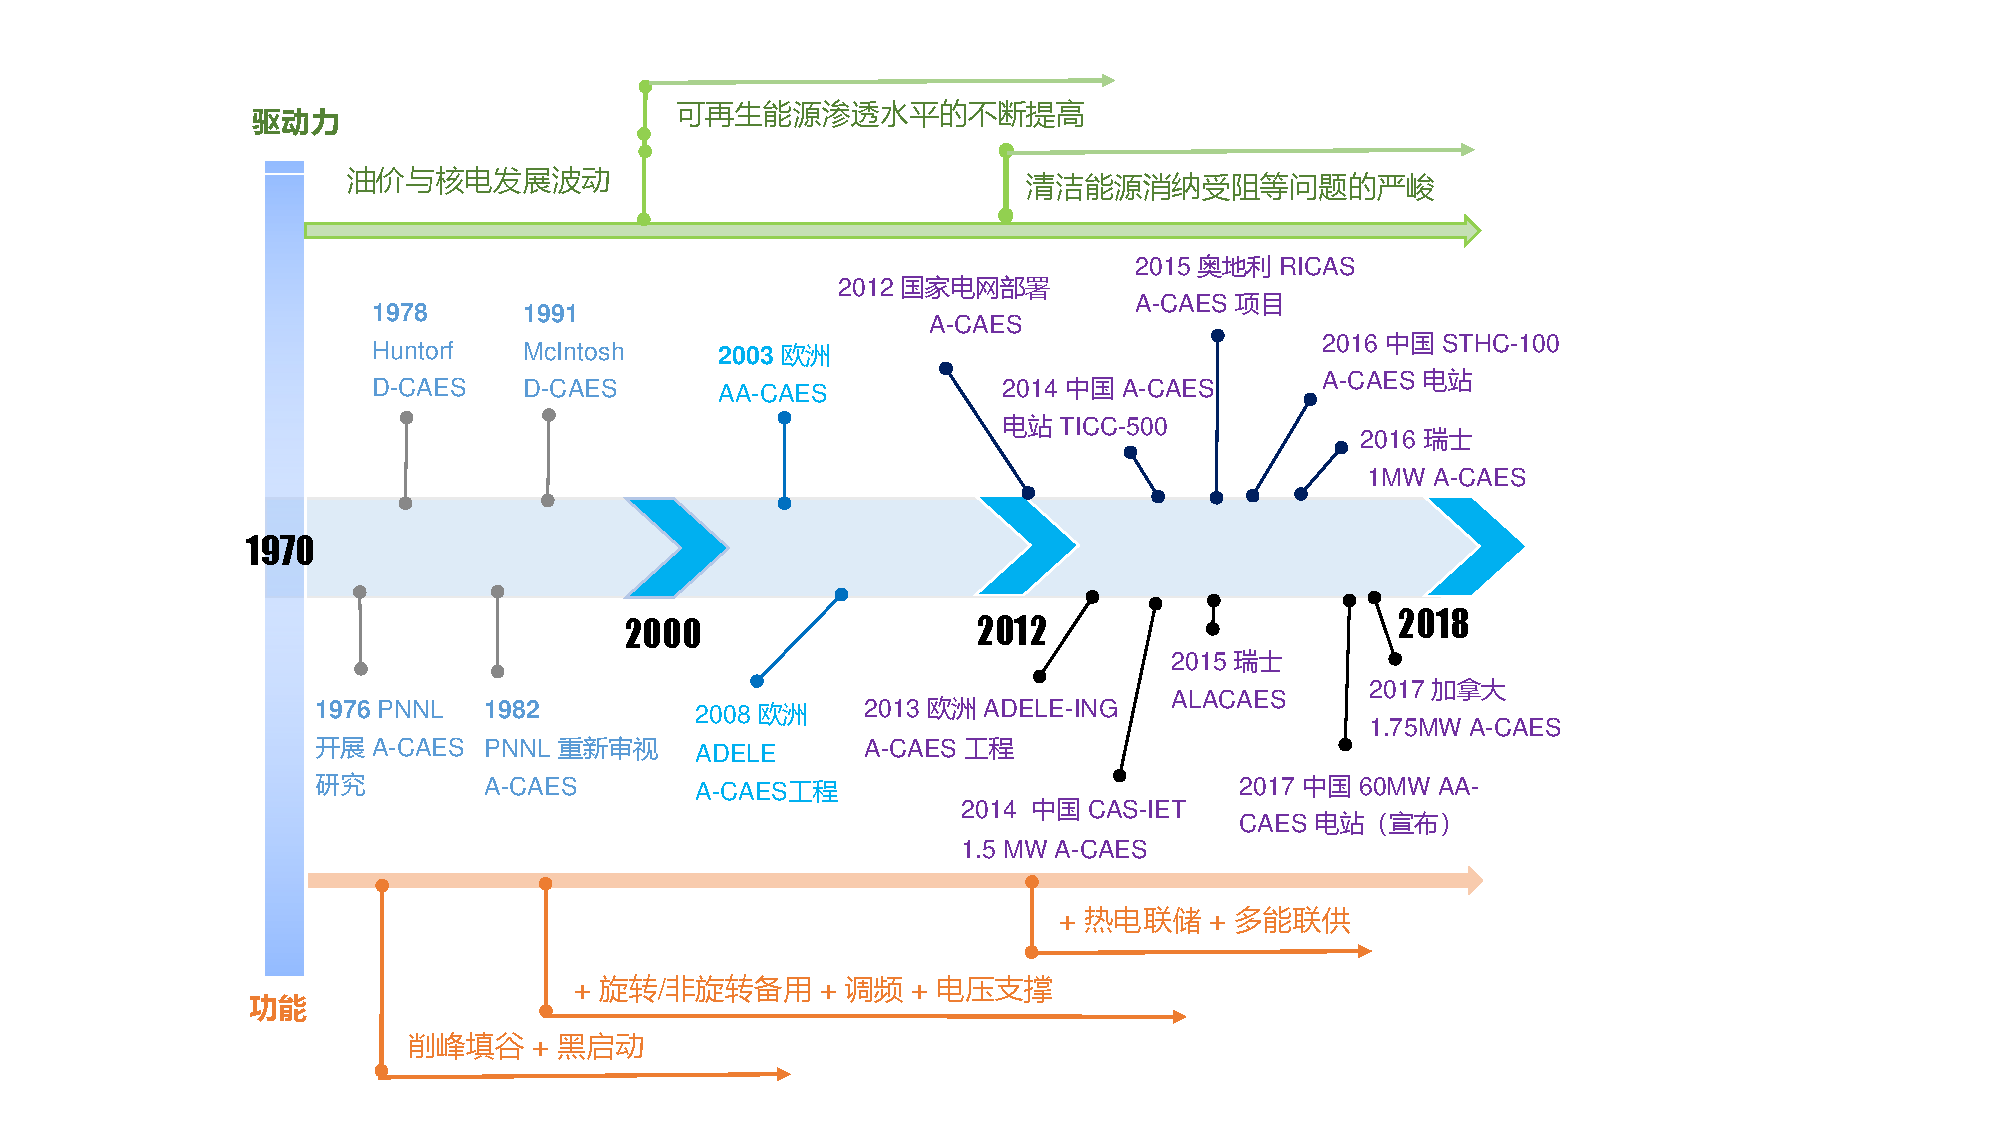
\includegraphics[scale=0.60]{figures/Chap1-4-CAES-History.pdf}
  \caption{A-CAES技术发展沿革(1970-2018)}
  \label{fig:CAES-History}
\end{figure}

\subsubsection{工程示范}
立足国内,多项~AA-CAES~示范工程有序推进,部分试验系统已开花结果。2012年10月,在国家电网支持下,清华大学联合中科院理化所、中国电力科学研究院开展AA-CAES 关键技术研究\cite{CAES-Review-17-Rui-salt}。2014 年3 月,中科院工程热物理研究所建成河北廊坊1.5MW先进CAES的集成实验系统,完成了~600~小时试验运行和性能测试\footnote{http://www.cas.cn/ky/kyjz/201404/t20140403\_4085514.shtml};同年12月,清华大学建成安徽芜湖 500kW AA-CAES实验系统TICC-500,在国内率先实现储能发电,电换电效率达41\%(初期实验效率33.3\%),综合能量效率达72\%~\cite{TICC-15,TICC-16}。2016 年8 月,清华大学在青海大学智慧微能源网示范园区投运100kW光热复合CAES试验系统STHC-100,并初步完成冷热电三联供试验~\cite{ST-CAES-17,ST-CAES-CN-16-Rui};同年12 月,中科院工程热物理研究所开展贵州毕节10MW级AA-CAES系统集成实验与研发平台的联合调试\footnote{http://www.etp.ac.cn/xwdt/kydt/201612/t20161213$\_$4720289.html}。2017年5月,国家能源局批复立项我国首个AA-CAES国家示范电站——江苏金坛盐穴压缩空气储能发电系统~\cite{CAES-Review-17-Rui-salt};同年7月,国家能源局批复立项我国首个以AA-CAES为核心的“互联网+” 智慧能源示范项目—— 无为高沟电缆基地智能微电网
\footnote{http://www.nea.gov.cn/136106972$\_$14887900533341n.pdf}。2018年3 月,国家能源局《2018 年能源工作指导意见》指出,"积极推进江苏金坛压缩空气储能项目,研究推进100MW压缩空气储能电站";2018年12月,金坛压缩空气储能项目开工建设
\footnote{http://www.escn.com.cn/news/show$\_$696396.html}。

放眼国际,德国、美国、加拿大、奥地利、瑞士等国纷纷宣布、设计或建设多座AA-CAES电站~\cite{CAES-Review-16-Polygeneration,CAES-Review-09,CAES-Review-16-Rui}。2003 年,欧盟委员会资助~AA-CAES~项目,旨在评估面向集中式、分布式及孤岛等应用场景的AA-CAES技术方案,并构建具有经济吸引力的概念型电站~\cite{AA-CAES-04}。2008 年,德国莱茵集团等启动~ADELE~ 项目,开展~AA-CAES~技术的可行性论证、概念设计及组件研发等工作~\cite{AA-CAES-07};2013年,莱茵集团进一步启动~ADELE-ING~项目,研究~AA-CAES~技术的工程特性并评估不同的系统方案\footnote{http://www.sccer-hae.ch/resources/SymposiumMay2015/Talks/SCCER2015-AdiabaticCAES-Zunft.pdf},筹划建设~ADELE~ 示范电站,设计容量达300MW/1000MWh,预计循环效率达66\%-70\%\footnote{2017年12 月,由中国盐业公司、清华大学等单位组成的考察团赴德国调研表明,该项目目前已被终止。}。 2013 年,美国PNNL 评估了Yakima 结合地热和盐穴储气的~AA-CAES~方案~\cite{AA-CAES-Patent-12} 及其技术经济性~\cite{CAES-PNNL-13}。2015 年,奥地利启动 RICAS2020 项目评估~AA-CAES~技术的性能与可行性,并聚焦于研发较具经济性的地下储气方案,同时构建移动式~AA-CAES~系统~\footnote{https://www.sintef.no/en/projects/ricas-2020-design-study-for-advanced-adiabatic-com/}。 瑞士~ALACAES~公司致力于研发面向~AA-CAES~的储热技术,采用隧道和洞穴储气方案评估了~AA-CAES~ 技术的环境经济潜力,于~2016~年在瑞士比亚斯卡建成了一座~1MW/MWh AA-CAES~示范系统~\footnote{https://alacaes.com/},并在文献~\inlinecite{AA-CAES-Demo-ALACAES-1,AA-CAES-Demo-ALACAES-2}中基于储热系统的实测数据及其它组件的预估性能,得出了63\%-74\%的电-电循环效率。2017 年5月,加拿大~NRStor~和~Hydrostor~公司开始联合研发大规模~AA-CAES~技术,目前正在加拿大戈德里奇建设一座基于盐穴储气~1.75MW/7MWh~AA-CAES试验电站~\footnote{https://www.energy-storage.news/news/canadian-firms-nrstor-and-hydrostor-partner-up-on-utility-scale-adiabatic-c}。

毋庸置疑,上述工程实践极大加强了面向新能源电力系统源、网、荷侧各应用场景的AA-CAES设计、建模、运行及运营等理论与方法的研究需求, 而分析AA-CAES独特的灵活性特点则是开展相应研究工作的前提。

%\subsection{新型灵活压缩空气储能系统}

\subsection{压缩空气储能系统的三类灵活特性}
\label{sec:flexibility-intro}
前已提及,独特的热力循环与设计理念赋予了AA-CAES多种灵活性,具体包括:1)以能量搬移与容量备用为核心的常规灵活性;2)以热电联供与热电联储为特点的供能灵活性;3)以机械输入与机械输出为内涵的接口灵活性。AA-CAES的常规、供能及接口等三类灵活性,为从源、网、荷三侧促进高比例可再生能源电力的可持续供应提供了新视角。

\subsubsection{常规灵活性:能量搬移与容量备用}
CAES的大容量特性及优良的动态特性使其具备了长时间的能量储存与搬移功能,以及良好的容量备用等灵活性支撑能力。实际运行表明,D-CAES电站具有启动速度快、爬坡率高、工作范围宽及运行模式灵活等优点\cite{CAES-Review-18-Rui-operation}。具体表现为:1)快速启动能力,3min—5min 可达70\%膨胀发电容量,10min 内实现满功率发电,5min 内实现满功率压缩~\cite{Huntorf-20-01};2)高爬坡率,如McIntosh 电站爬坡率约为18MW/min, 高于典型燃气轮机约60\%~\cite{CAES-Alabama-06};3)宽工况运行能力,如McIntoch 电站透平机械设计及控制方案提供方Dresser-Rand 公司拥有的SMARTCAES在发电和压缩环节均可实现25\%-100\% 负载运行\footnote{http://www.dresser-rand.com/industries/energy-environment/compressed-air-energy-storage/};4)灵活的运行模式,既可以超前功率因数运行的电动机模式压缩储能和提供无功,亦可以单位或滞后功率因数运行的发电机模式膨胀释能,抑或是以同步调相模式提供动态无功支撑~\cite{CAES-Reactive-13,CAES-Reactive-18-LGK}。 上述优良动态特性使~D-CAES~电站具备了调频、备用、无功调节及黑启动等功能,可为电网相关服务提供灵活性支撑,也为D-CAES电站的市场运营提供了多个收益源,有利于提高其竞争力与经济性。

\begin{figure}[htp] % use float package if you want it here
  \centering
  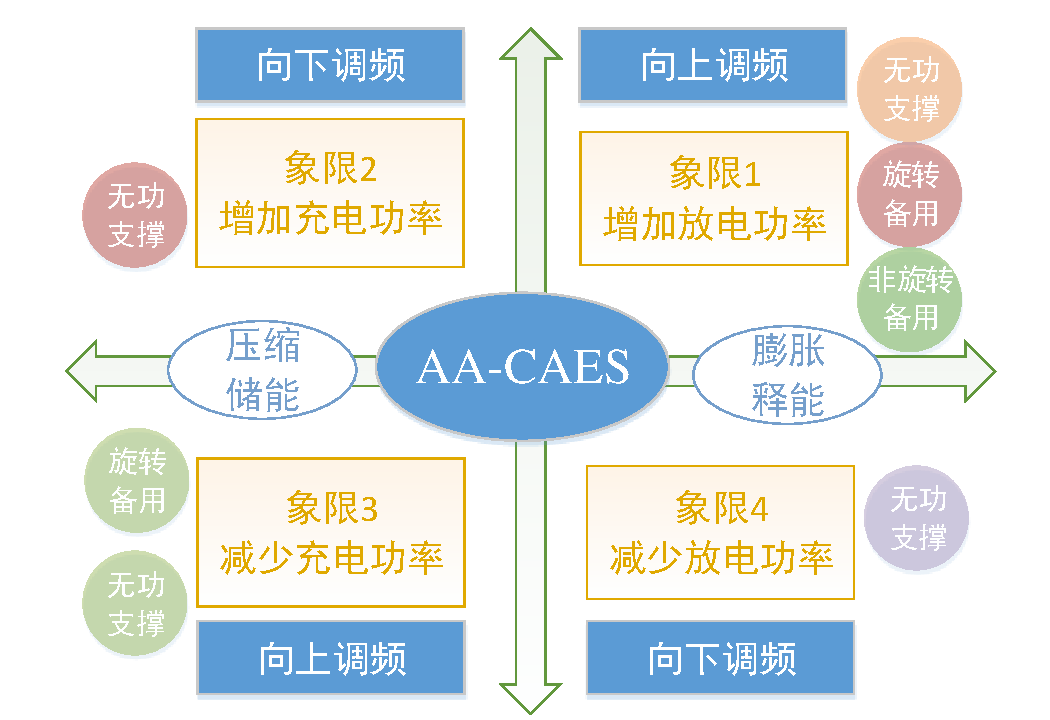
\includegraphics[scale=0.60]{figures/Chap1-2-CAES-AS-Overview-2.pdf}
  \caption{AA-CAES 辅助服务功能示意图}
  \label{fig:CAES-AS-Overview}
\end{figure}

不同于D-CAES电站,AA-CAES采用蓄热系统代替燃料补燃,压缩机与膨胀机一般不共轴\footnote{D-CAES一般采用共轴方案的原因在于其设计理念源于内含共轴压缩机与膨胀机的燃气轮机。},从而能够减少压缩、停机(静置)、膨胀模式间的切换时间,提高了压缩环节的响应速度,具有比常规D-CAES电站更为优良的调频、旋转备用等辅助服务特性~\cite{ESS-Model-14},如图~\ref{fig:CAES-AS-Overview} 所示。以调频为例,当电网频率下跌时,AA-CAES电站可通过增加膨胀(发电)功率或减少压缩(充电)功率为系统提供向上调频容量;当电网频率过高时,AA-CAES 电站可通过减少膨胀功率或增加压缩功率为系统提供向下调频容量。同时,AA-CAES电站在压缩储能与膨胀释能过程中均可为电网提供旋转备用容量,在膨胀释能过程中还可提供非旋转备用容量。此外,AA-CAES电站在压缩和膨胀过程中的无功支撑能力使其能为电网提供一定的无功支撑 \cite{CAES-Reactive-18-LGK}。

需要说明的是,1)与电池储能不同,AA-CAES的调频、备用容量等将受到其蓄热系统、储气系统及供能特性的影响\cite{AA-CAES-Reserve-LYW-18};2)由于蓄热系统(及换热器)的传热动态一般比燃烧过程慢,采用蓄热系统代替天然气补燃环节后可能会降低AA-CAES在膨胀释能过程的响应速度\footnote{部分文献对此观点不一致,如文献\inlinecite{AA-CAES-Reserve-LYW-18}认为蓄热系统会比补燃环节更易提高响应速度。}。

\subsubsection{供能灵活性:热电联储与热电联供}
\label{sec:flexibility-poly-generation}
AA-CAES包含压缩机、膨胀机、换热器、蓄热系统、储气库等组件,各组件的热力学特性紧密耦合。换热器及蓄热系统的存在使AA-CAES电站可利用富余的压缩热能(或外部扩展热源)供热,具备了热电联供特性,提高了综合能量效率。AA-CAES 电站的电能存储与热量存储特性赋予其热电联储能力,为其提供了良好的供能灵活性,适宜在分布式多能联供场景应用,如区域综合能源系统中实现热电协同调控~\cite{Trigen-mCAES-15,CAES-Alberta-14},进而提升新能源电力的渗透水平。

AA-CAES具备的结构层面的灵活扩展能力,可以增强其热电联储与热电联供能力。通过辅助电加热单元~\cite{Hybrid-CAES-14}、 光热收集单元~\cite{EH-CSP-17-Rui,Wind-Solar-CAES-12-Xu} 等外部扩展热源,扩展后的系统具有更强的热电联供与联储能力,提升了AA-CAES的供能灵活性。图~\ref{fig:ST-CAES-Hub} 给出了一种具有外部扩展热源的AA-CAES系统结构,可以实现灵活的热电联供与热电联储功能,是一种典型的热电清洁能量枢纽。文献~\inlinecite{ST-CAES-CN-16-Rui,ST-CAES-17,ST-CAES-CXT-18} 所构建的光热复合压缩空气储能系统即为一种采用槽式集热辅助单元的多能联供型AA-CAES能量枢纽。此外,文献~\inlinecite{High-Temp-CAES-17} 也给出了一种结合光热或低中温废热的AA-CAES 系统,在增强供能灵活性的同时,可以降低系统成本。

\begin{figure}[H] % use float package if you want it here
  \centering
  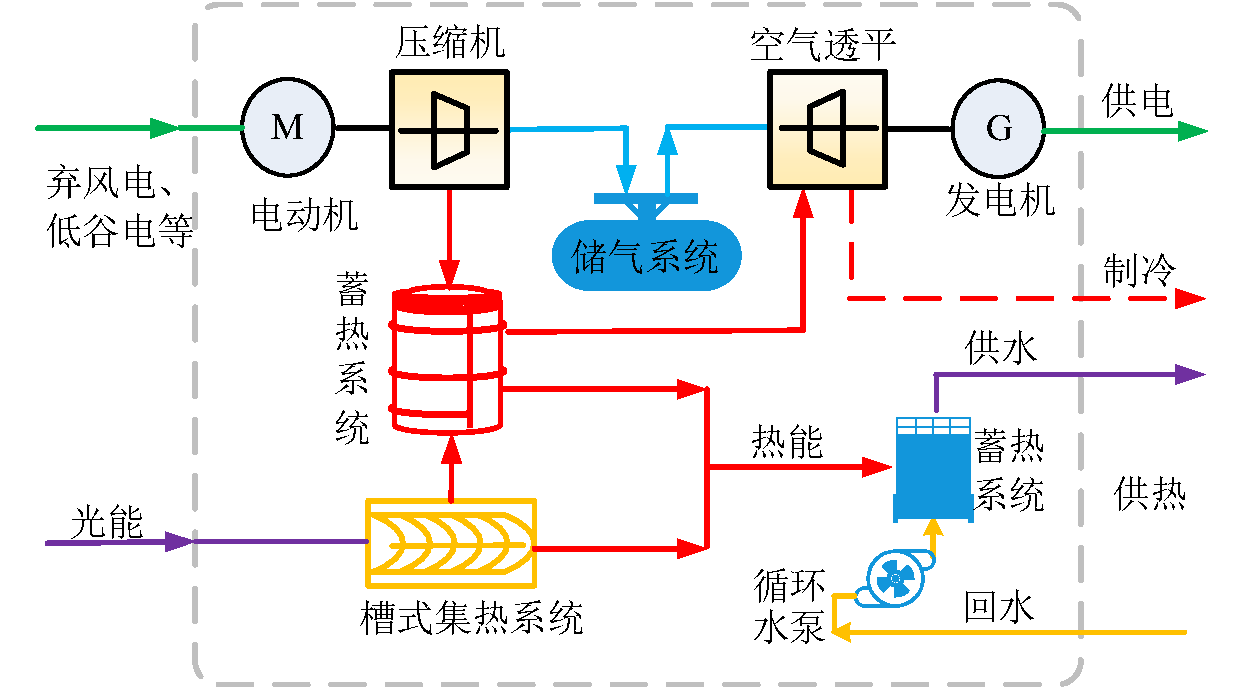
\includegraphics[scale=0.50]{figures/Chap1-3-ST-CAES-Hub.pdf}
  \caption{典型AA-CAES能量枢纽的结构}
  \label{fig:ST-CAES-Hub}
\end{figure}

事实上,AA-CAES可引入的电加热、光热等结构,本质上可视为接口灵活性。但是,本文关注的接口灵活性特指AA-CAES整体与新能源电力系统的机械能(非电)输入与机械能(非电)输出接口,而增设补热环节等改善AA-CAES 多能联供能力的结构灵活性被纳入供能灵活性。

\subsubsection{接口灵活性:机械输入与机械输出}
不难发现,图~\ref{fig:AA-CAES-principle-abs}中~AA-CAES~的输入与输出端分别采用电动机与发电机实现与电力系统的电能形式接口。事实上,我们可以直接采用风能等机械能驱动AA-CAES中的压缩机(省去压缩机前面的电动机),如文献~\inlinecite{Thesis-Zhangyuan,WT-CAES-Fea-15,CA-WT-16,Thesis-Zhangyi}设计的风-储集成系统;同时,也可直接利用AA-CAES 透平膨胀机输出的机械能(省去膨胀机后面的发电机),无需将其转化为电能,如法国MDI公司的压缩空气动力汽车AIRPod\footnote{MDI: Motor Development International.}。 如此,我们可以有效地利用风能直接驱动压缩机或直接输出机械能,实现风-储集成设计,从而有望降低风机存在的风速与风电输出功率之间的瞬时强耦合性以及新能源电力系统对灵活性资源的需求。本文将AA-CAES的这一灵活特性称之为接口灵活性。相比于AA-CAES,电池等其它储能技术必须以电能输入与电能输出作为其与电力系统的接口,其灵活性较差。

\begin{figure}[htp] % use float package if you want it here
  \centering
  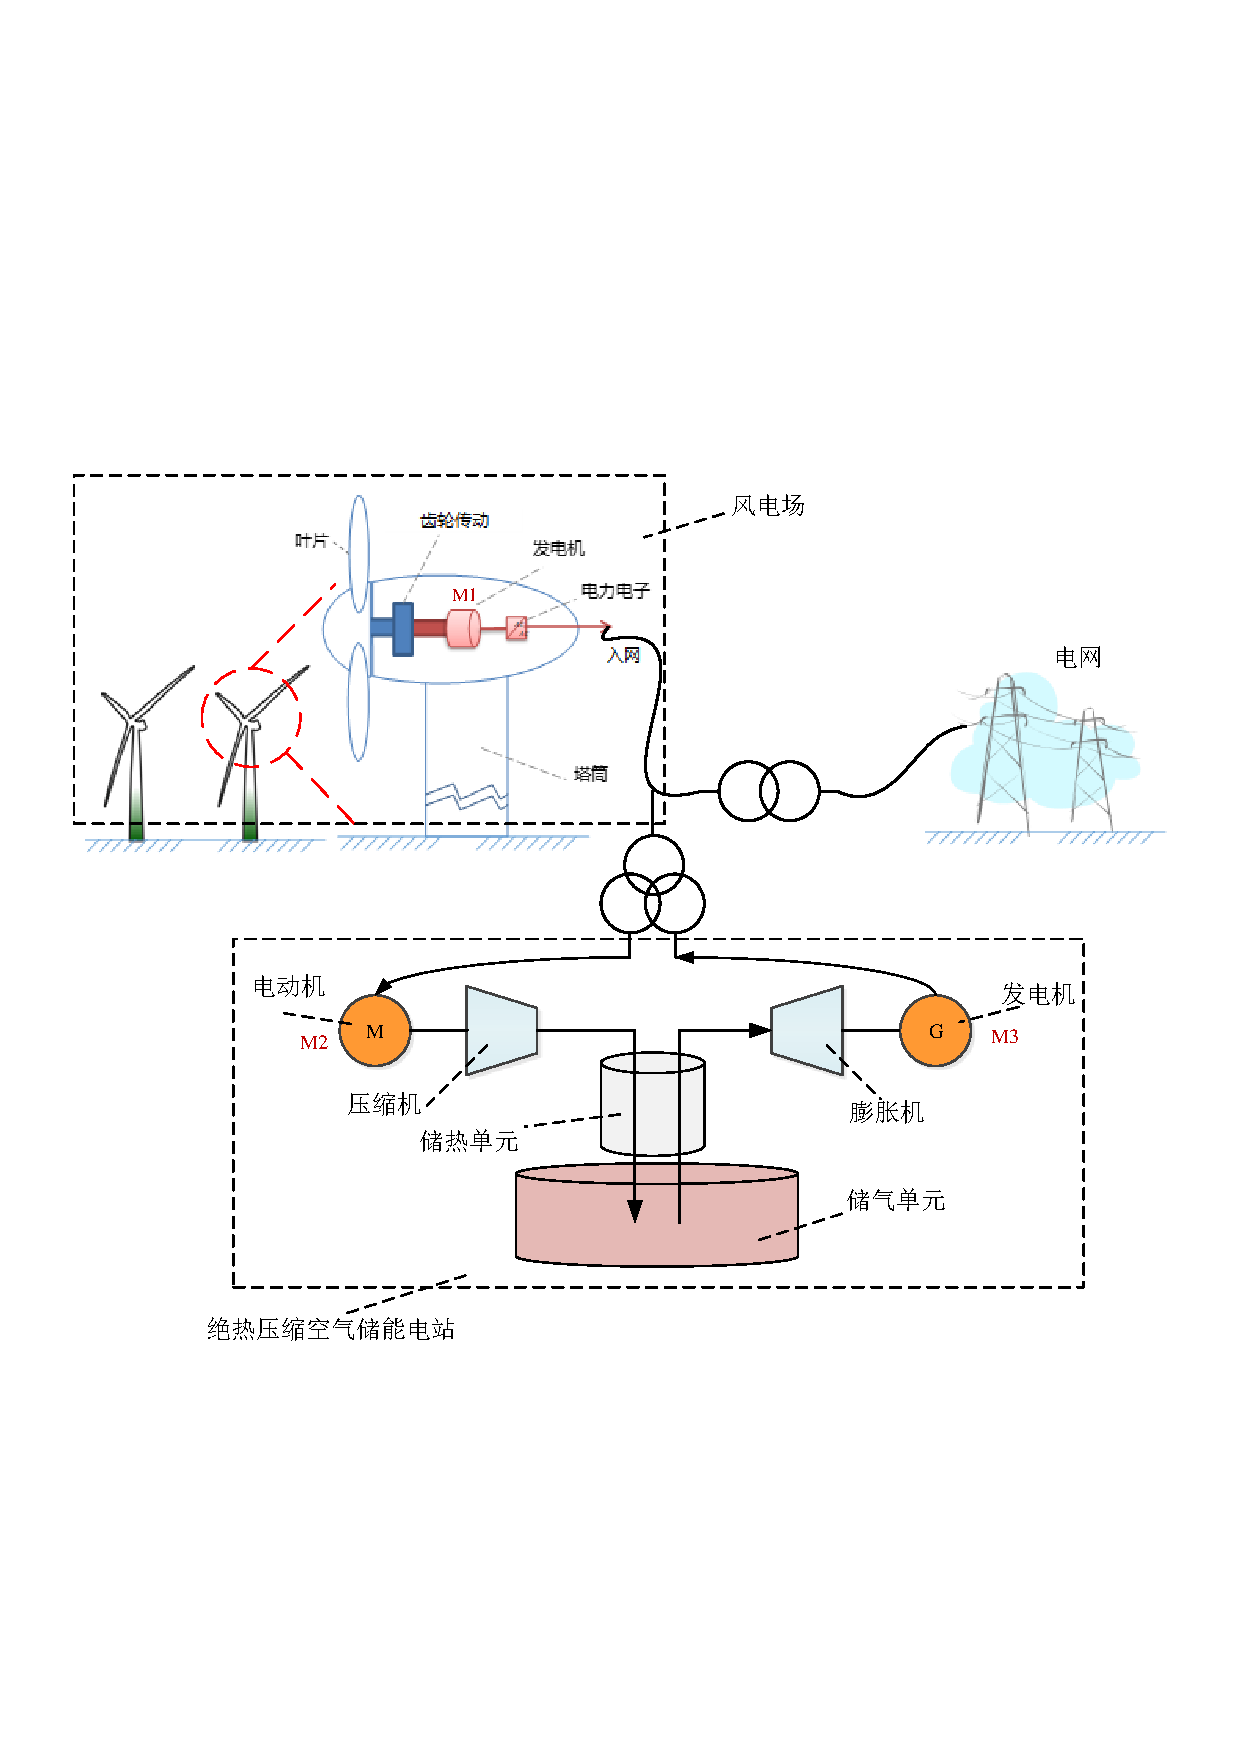
\includegraphics[scale=0.75]{figures/Chap1-5-AA-CAES-Stru-Flex.pdf}
  \caption{风-储协同系统中的AA-CAES接口灵活性示例}
  \label{fig:AA-CAES-Stru-Felixibity}
\end{figure}

以图~\ref{fig:AA-CAES-Stru-Felixibity}~所示的风电场与储能(AA-CAES)混合系统的经典配置结构为例, 我们分析需挖掘接口灵活性的典型场景。由于AA-CAES储能电站的压缩机及膨胀机需分别配设电动机与发电机,风-储混合系统一般至少含有三个电机~M1-M3。然而,三个电机均存在一定程度的容量浪费问题,具体地:1)风机内部的发电机M1 因可利用风能的大小在风速低于风机额定风速时存在着不同程度的容量浪费问题(风速越低问题越严重);2)M2在AA-CAES膨胀释能过程与静置时存在100$\%$ 的容量浪费;3)M3在AA-CAES压缩储能过程与静置时存在100$\%$的容量浪费;4)在风电上网不受限时段,由于AA-CAES储能系统无需运行,M2与M3完全静置。换言之,风-储(AA-CAES)混合系统中M2与M3的利用率远低于应用于负荷侧从电网进行储能的AA-CAES电站。若能挖掘AA-CAES的接口灵活性,直接采用风机叶片的(富余)机械能驱动压缩机以及采用膨胀机(与风机叶片共同)驱动风机内部的发电机M1,实现风-储集成设计,则有望省下风-储协同系统中AA-CAES包含的电动机M2与发电机M3,从而在改善M1-M3的容量浪费问题的同时,平滑了风电出力的波动性,从源头上赋予风电可调度性,降低了电力系统为实现高比例新能源电力供应而新增风电装机容量时(可参见图\ref{fig:Wind-Installment-Capacity})对灵活性资源的需求。

\subsection{压缩空气储能系统的热力学特性建模与仿真}

AA-CAES具有的常规、供能及接口灵活性使其既可应用于电力系统削峰填谷~\cite{CAES-MultiValue-11,CAES-Princeton-08}、频率调节~\cite{CAES-Congession-09,CAES-Reserve-11}、旋转备用~\cite{CAES-Congession-09,CAES-Reserve-11}、无功支撑~\cite{CAES-Reactive-13,CAES-Reactive-18-LGK}、黑启动~\cite{Huntorf-20-01}等场景,亦可应用于热电联供系统或分布式能源系统~\cite{CAES-Review-18-Rui-operation,CAES-IES-16-Rui,Trigen-mCAES-15,CAES-Alberta-14}。 在上述典型应用场景中,AA-CAES将可能频繁处于宽工况(off-design)运行条件,导致内部压缩机、换热器、膨胀机等组件的部分负载运行(part-load)\footnote{为了避免歧义,本文称AA-CAES系统级的非额定运行为宽工况运行,称内部组件级的非额定运行为部分负载运行。}, 从而引起~AA-CAES~整体运行性能的变化。同时,压缩机、换热器、膨胀机、储热罐、储气室等组件间的热力学特性高度耦合,彼此之间相互影响。在此背景下,建立计及组件部分负载运行特性的宽工况热力学仿真模型对分析~AA-CAES~内部的热力学特性及外部的供能特性具有重要意义。

当前在AA-CAES热力学特性仿真分析方面,一般采用固定效率模型来描述内部组件的功-能转换关系,也有部分文献研究了计及部分负载运行特性的仿真模型。文献\inlinecite{A-CAES-Therm-12}指出二次曲线描述质量流率增减(部分负载运行)导致的压缩机与膨胀机效率变化特性, 并研究了换热器的关键参数对AA-CAES系统性能的影响。文献\inlinecite{Compressor-thermo-02}给出了燃气轮机内部的压缩机与膨胀机在部分负载运行时压缩比、膨胀比及等熵效率随质量流率的解析关系。文献\inlinecite{A-CAES-Dynamic-17}利用该解析式,建立了填充床储热型AA-CAES的热力学仿真模型;然而,该文对储气库与壁面换热问题的处理过于简单,同时未考虑换热器的部分负载特性。文献\inlinecite{CAES-Discharge-16}基于文献\inlinecite{Compressor-thermo-02}中的压缩机及透平的部分负载特性曲线,研究了D-CAES电站透平侧的常压及滑压运行模式;但该文采用等温模型刻画储气库的动态特性,未能计及空气进出储气库以及储气库与周围环境间传热引起的库内空气温度变化对透平侧热力学特性的影响。

在首级压缩机的压缩热供暖的假设下,文献\inlinecite{CAES-CCHP-off-design-18}分析了额定运行工况下压缩机与膨胀机在常压、滑压等运行模型时的热电联供特性,但未考虑压缩机、膨胀机及换热器等组件的部分负载特性。基于额定运行工况的假设,文献~\inlinecite{Exergy-storage-17}建立了储气库动态模型,并评估了储气库的㶲存储能力。文献\inlinecite{Ene-Exe-ACAES-17}基于定压储气库模型,研究了微型压缩空气储能在额定运行工况下的能量特性及㶲特性。文献~\inlinecite{TES-Eff-CAES-13}分析了基于额定运行工况的AA-CAES中储热系统的热力学动态对AA-CAES特性的影响,但未考虑宽工况及多能联供。文献\inlinecite{Heat-mass-transfer-11}给出了顺流、逆流及管壳式等不同种类换热器的部分负载运行特性,文献~\inlinecite{A-CAES-Dynamic-17}利用该模型研究了填充床储热型AA-CAES的宽工况运行特性。文献~\inlinecite{TES-CSP-review-13} 给出了适应于集中式光热电厂的储热技术及运行模型,为分析AA-CAES中储热系统的能量及㶲特性提供了参考。文献~\inlinecite{Model-AA-CAES-10} 研究了一典型四级压缩— 两级膨胀~AA-CAES~系统的额定设计工况运行特性,并考虑了储气库温度与压力变动对运行性能的影响,但未计及压缩透平机械的部分负载运行特性,也未考虑运行模式对AA-CAES的影响。

总之,当前在计及压缩机、膨胀机、换热器等组件的部分负载特性以及储气库与储热系统动态特性的AA-CAES宽工况热力学特性仿真方面的研究尚不充分,难以有效支撑面向电力系统与综合能源系统应用的AA-CAES各灵活性应用场景的建模分析、调度运行及市场运营等问题。

\subsection{面向电力系统的压缩空气储能系统建模及运行}
AA-CAES技术在电力系统的应用推广离不开相应的调度运行及市场运营方法的支撑。然而,正如第\ref{sec:research-state-engineer}节评述可知,当前AA-CAES技术尚处于工程示范阶段,国际上对其运行建模、调度运行及市场运营方面的研究极为匮乏,但已有较多文献探讨了D-CAES电站的相关建模与分析方法。尽管AA-CAES在一定程度上类似于D-CAES电站,但换热器及蓄热系统赋予的内部空气压力势能与压缩热能在压缩储能(膨胀释能)过程的解耦存储(耦合释能)特性,使得AA-CAES的建模分析拥有独特之处。

\subsubsection{调度运行}
在AA-CAES储能电站的运行及运营过程中,电网、电厂或第三方主体等投资者最为关心的问题之一即为经济性。文献\inlinecite{CAES-State-11}建立了D-CAES电站状态空间模型以监测储气库运行状态,并在给定地理条件下评估了压缩机容量、透平容量、充电时间、放电时间等参数配置对系统经济性的影响。文献\inlinecite{CAES-MultiValue-11} 以最大化日前电量市场和辅助服务市场的套利为目标,分析了不同商业模式下~D-CAES~电站在法国电力市场中的运行经济性。文献\inlinecite{ERCOT-11}针对ERCOT电网的研究表明,当风电和光伏容量渗透水平达80\% 时,CAES等大规模储能技术是维持弃光、弃风率低于10\% 的必要手段。文献\inlinecite{BulkESS-Benefit-15}评估了D-CAES电站在降低市场电价与电力系统生产成本方面的潜力。国际能源气候环境领域知名学者,哈佛大学David Keith教授在文献\inlinecite{ESS-Decarbon-David-15}中从功率投资和容量投资成本角度评估了储能电站的经济性,指出尽管AA-CAES的效率低于其它大规模储能技术,但在新能源电力系统深度低碳化及当前的投资现状下,AA-CAES是最具经济性的大容量清洁储能技术。

在调度运行方面,文献\inlinecite{SCUC-CAES-12}采用等效电池模型\footnote{本文所指的等效电池模型为采用充电效率及放电效率等描述储能水平的(简化)效率模型。}描述D-CAES电站的运行特性,研究了含D-CAES 电站的电力系统机组组合问题,从节点边际电价、削峰填谷、输电线阻塞管理、弃风及环境效益等方面分析了D-CAES电站对电力系统运行的影响。文献\inlinecite{ESS-Opt-Place-13}采用概率最优潮流模型,计及储能电站对市场电价的影响,研究了高风电渗透水平下电力系统中D-CAES电站的运行策略;算例表明,在风电电量渗透水平为20\%时仅靠电量套利不足以平衡D-CAES电站的运行成本,需要新能源容量补贴等其它收益;当风电电量渗透水平达45\% 时,通过电价套利可确保电站经济性。针对含D-CAES电站的电力系统机组组合和经济调度问题,文献\inlinecite{CAES-Value-Ireland-17}分别采用等效电池模型与计及储气库动态对压缩机和透平运行影响的热动态模型,评估了D-CAES电站对消纳爱尔兰电力系统中风电的作用,并指出等效电池模型所得结果过于乐观。文献~\inlinecite{CAES-Bilinear-17} 基于CAES储气库压力与温度的详细动态模型,建立了具有较高准确度与较低计算复杂度的储气库双线性模型;进一步,文献\inlinecite{CAES-Bilinear-UC-17}将该双线性模型应用于含D-CAES电站的电力系统机组组合问题。

文献\inlinecite{Opt-Alloc-ESS-15}研究了电量和辅助服务联合市场中D-CAES电站的最优配置方案,对比了配置储能与扩建输电线两种方案,并构建了经济性评估指标,以为储能投资者的决策提供参考。文献\inlinecite{CAES-Micro-Bilevel-16}提出了含D-CAES电站的孤岛微电网双层规划方法,上层为定容问题,下层为含旋转备用需求的机组组合问题。然而,上述文献并未计及D-CAES电站宽工况运行特性的影响等实际运行问题,研究结论过于乐观。文献\inlinecite{CAES-Real-Time-Dispatch-LYW-18}研究了含D-CAES 电站的电力系统日前日内协调调度策略,实现了D-CAES电站电量及旋转备用容量的协同优化调度。文献\inlinecite{CAES-Reactive-13}研究了D-CAES电站作为调相机的可行性,指出D-CAES支撑失速型风机无功的优势。文献\inlinecite{CAES-Reactive-18-LGK}探讨了AA-CAES系统的调相运行模式,为计及AA-CAES的无功支撑能力构建电力系统优化调度模型提供了初步依据。文献\inlinecite{AA-CAES-Reserve-LYW-18}详细分析了AA-CAES电站的备用特性,建立了计及AA-CAES备用特性的电力系统调度方案。但文献~\inlinecite{AA-CAES-Reserve-LYW-18}与\inlinecite{CAES-Real-Time-Dispatch-LYW-18}中的相关模型过于复杂,难以有效刻画系统宽工况运行对内部组件部分负载特性以及对外部供能特性的影响。

综上,当前研究大多采用等效电池模型描述CAES的运行特性,未考虑运行过程中的宽工况特性对系统对外运行性能的影响,导致运行调度策略过于乐观。同时,上述研究大多针对传统D-CAES电站,较少涉足AA-CAES电站的调度运行问题,不利于发挥AA-CAES的常规灵活性对新能源电力系统的支撑作用。

\subsubsection{市场运营}
目前全球储能市场中抽水蓄能电站的装机容量约占99\%以上,其市场运营技术较为成熟。当前,我国抽水蓄能电站运营一般采用容量电价和电量电价
\cite{PHP-Market-CN-06,PHP-Price-CN-07}。 类似抽水蓄能电站,AA-CAES电站在建设初期可由电网、电厂或第三方投资主体投建,建成后可以独立运营主体等形式参与市场运营。然而,国家能源局在批准江苏金坛AA-CAES示范项目时并未给出其运营模式,因此有必要重视AA-CAES电站的市场运营技术,以为实际AA-CAES电站的商业运行提供参考。

大容量及小容量CAES电站可分别以价格影响者(Price-maker)与价格接受者(Price-taker)的角色参与电力市场电量、辅助服务、实时交易等运营
\cite{CAES-BidOff-Curve-17}。 作为价格接受者,CAES电站的压缩储能与膨胀释能行为不影响市场电价,因此可通过预测市场电价实现储能电站的市场运营\footnote{市场参与主体以Price-taker参与市场竞标的问题又称为Self-scheduling。}。作为价格影响者,大容量CAES电站可以储能与释能电价及对应的电量为竞标标的,通过参与电力市场的策略竞价影响市场价格,进而最大化运行收益\cite{Thesis-Shafiee}。

文献\inlinecite{Operation-CAES-Spot-09}采用价格接受者机制,给出了较具实际意义的D-CAES电站的运行策略, 以克服电价预测误差等带来的预估收益乐观等问题。文献\inlinecite{Value-Arbit-ESS-Eurpoean-16}研究了D-CAES电站在欧洲电力市场的套利策略,并指出在煤炭占比较大的电力市场中CAES电站具有较大的套利收益。为规避价格预测误差带来的套利风险,文献\inlinecite{Risk-Bid-Off-CAES-17}提出了基于信息鸿沟决策理论的D-CAES电站竞价策略,给出了价格处于最大变化区域时确保最低利润的鲁棒竞价策略,以及在有利价差下获取最高利润的乐观策略。文献\inlinecite{Robust-Bid-Off-CAES-18}计及了电力市场价格的不确定性,采用等效电池模型建立了面向日前电力市场的商业运营D-CAES电站的鲁棒竞标策略。

事实上,文献\inlinecite{Risk-Bid-Off-CAES-17,Robust-Bid-Off-CAES-18} 均基于等效电池模型分析D-CAES电站的竞价策略,并未计及宽工况运行下内部组件的部分负载特性对套利收益的影响。文献\inlinecite{CAES-Reserve-Bid-Therm-16} 考虑了压缩机、透平的部分负载效率特性,研究了D-CAES电站在日前电量和备用联合市场中的竞价策略;研究表明,在电量市场中不考虑部分负载运行特性时等效电池模型具有可接受的准确度,但当D-CAES电站同时参与日前电量和备用市场时等效电池模型具有明显误差\cite{CAES-Reserve-Bid-Therm-16}。然而,文献\inlinecite{CAES-Reserve-Bid-Therm-16}假定D-CAES是价格接受者,不影响市场价格,同时也没有考虑换热器等AA-CAES必备组件的部分负载运行特性。

综上,当前研究主要面向目前已实现商业运营的D-CAES电站的调度运行及市场运营问题,鲜有文献针对正在建设的AA-CAES电站的运行调度、市场运营展开研究,也很少计及AA-CAES内部特有的换热器及蓄热系统等组件的部分负载特性与热力学动态特性。同时,大多研究以价格接受者机制研究CAES电站的市场运营,难以适用于大容量AA-CAES储能电站接入电网对市场电价的影响特性,导致计及宽工况运行特性的AA-CAES灵活性建模及调度运行相关理论与分析方法的缺乏。从而,不利于挖掘AA-CAES具有的以能量搬移及容量备用为特征的常规灵活性对实现可持续的高比例可再生能源电力供应目标的支撑作用。

\subsection{面向综合能源系统的压缩空气储能系统建模及运行}
与D-CAES不同,AA-CAES采用蓄热系统(或外部扩展热源)实现了空气压缩热能(或环境余热)的回收和再利用,蓄热系统中的剩余热量或透平的高温乏气可进一步通过“温度梯级利用”实现供热,透平低温排气或辅助热驱动制冷机后亦可提供冷量\footnote{透平乏气(排气)的温度可通过膨胀释能阶段换热器换热量的大小来调节,若换热量足够多,透平入口空气温度高,相应的排气温度也高,若换热不充分,透平入口空气温度低,相应的透平排气温度也较低。},从而提升了能量综合利用效率~\cite{Trigen-mCAES-15,CAES-Alberta-14,TES-Eff-CAES-13}。AA-CAES电站的热电联供、热电联储能力使其在热电综合能源系统中得以应用,具体主要聚焦于两方面,一是小型分布式多能联供系统,二是大型热电联供电站。

\subsubsection{小型分布式多能联供系统}
在小型分布式CAES多能联供可行性方面,文献\inlinecite{CAES-CCHP-Exergy-17}开展了由风电、燃气轮机、储气库、吸附式制冷机等构成CAES冷热电三联供系统的能量及㶲分析。文献~\inlinecite{Mul-Obj-CAES-CCHP-17}对CAES多能联供系统进行了㶲经济分析,并基于微分演化算法权衡总体㶲效率及生产成本。文献\inlinecite{Tri-CAES-TES-12} 提出了一种基于储热技术及D-CAES技术的分布式能源系统,并进行了效率评估。文献~\inlinecite{Thermo-WSCAES-17}提出了一种基于D-CAES的风-光-储混合多能联供系统,采用光热补热实现电能和热能的稳定供应,并结合有机朗肯循环实现不同品位热能的综合梯级利用。文献\inlinecite{mCAES-Heating-Cooling-10}采用热力学第一定律和第二定律对比分析了绝热、近似等温等模式下,基于D-CAES的小型分布式供能系统的运行特性,指明了小型D-CAES 系统应用于分布式能源领域的可行性。文献
\inlinecite{TES-Eff-CAES-13}通过典型系统参数分析指出,AA-CAES达到最大发电效率时尚有剩余压缩热能可用于供热。

文献\inlinecite{Subcool-CAES-17}构建了一种新型的过冷式(sub-cooled)AA-CAES系统,其电–电转换效率及电–热转换效率分别达30.6\%与32.3\%,并分析了其在接入小型区域供热管网以及为电网提供辅助服务的潜力。文献\inlinecite{Trigen-mCAES-15,Tri-CAES-Model-17}提出了基于AA-CAES的冷热电三联供系统,并分别进行了热动态和经济性分析;该系统采用压缩热提供热水,利用透平乏气制冷。文献~\inlinecite{Thesis-Zhangyuan}给出了AA-CAES系统供电、热电联供模式下的分布式能源系统模型,分析了系统供能模式与透平机械效率、压比、换热器传热系数等参数的关联性。为提高AA-CAES系统的供能经济性,文献\inlinecite{ST-CAES-CXT-18}提出了一种分布式光热复合压缩空气储能系统,采用压缩热供暖,利用槽式解热系统收集的热能供透平发电使用,并进行了额定工况下的系统性能分析。文献\inlinecite{Hybrid-CAES-14}提出了一种利用富余风电加热储热罐的混合热型AA-CAES系统,旨在解决压缩机排气温度(远)低于储热介质最高温限造成的储热介质热容量浪费问题,以期提升单位工质(高压空气)做功能力。

%总体而言,当前研究均针对AA-CAES额定运行工况,未计及其非额定工况等实际运行问题。同时,在小型AA-CAES分布式多能联供系统调度运行及市场运营方面的研究也不充分。

\subsubsection{大型热电联供系统}
在CAES接入供热管网构建大型热电联供枢纽电站方面,文献\inlinecite{CAES-DES-Exerg-14}提出采用蓄热系统收集CAES压缩热的方案,并将储热罐接于区域供热管网以供应商业及居民热负荷;㶲及㶲经济分析表明,配置储热罐的CAES电站作为热电联储系统及热电联供电站满足多能流需求的方案具有可行性。文献\inlinecite{CAES-Distri-Heat-David-13}提出了一种新型CAES结构(Distributed CAES),通过将压缩机配置于供热管网热负荷附近以满足供热需求,从而利用Distributed CAES作为能源集成站耦合区域热网和电网。进一步,文献\inlinecite{CAES-Heat-Export-14}分析了Distributed CAES 电站的热动态特性,文献\inlinecite{CAES-Alberta-14}利用Alberta 实际市场数据分析了Distributed CAES 实现电力套利的经济性,并研究了热负荷、储气室容量、透平压缩比及压缩空气管道对Distributed CAES经济性的影响。文献\inlinecite{CAES-IES-16-Rui}建立了计及热动态特性的AA-CAES多能互补模型,采用富余压缩热供热,用AA-CAES作为能量枢纽耦合电网和区域热网,发挥多能协同效应。

需要说明的是,无论是针对小型分布式多能联供系统,还是大型热电联供电站,当前研究并未给出AA-CAES热电联供时不同能流间的相互制约关系,对热电联供型AA-CAES同时参与热电协同调度运行及市场运营等问题的研究比较匮乏,不利于挖掘AA-CAES具有的以热电联供与热电联储为核心的供能灵活性对实现可持续的高比例可再生能源电力供应目标的支撑作用。

\section{研究目标及主要工作}
\label{sec:mind-work}
\subsection{研究目标}
新能源电力系统的可持续发展越来越多地依赖于系统中的灵活性资源,而高效灵活的储能技术是向电力系统注入灵活性的有效方式,并在电源侧、网络侧及负荷侧日益得到应用。AA-CAES是一种可灵活部署于源-网-荷侧的清洁储能技术,具有能量搬移与容量备用的常规灵活性、热电联供与热电联储的供能灵活性,以及机械输入与机械输出的接口灵活性等独特优点。本文以挖掘AA-CAES的这三类灵活性为目标,旨在系统研究以储能形式应用于电网侧的先进绝热压缩空气储能电站、以能量枢纽形式应用于负荷侧的先进绝热压缩空气灵活负荷、以风储集成形式应用于电源侧的内嵌先进绝热压缩空气储能的灵活风机的设计、建模、运行及运营方法,以充分发挥AA-CAES独特的储能循环对新能源电力系统的支撑作用。

事实上,无论以何种形式应用,在新能源电力系统中的AA-CAES需实现宽工况运行。只是源、网、荷各侧因其它灵活性资源的差异及实现形式的差别,存在的宽工况运行程度不同而已。这种外界应用导向的宽工况运行条件要求,造成了AA-CAES内部能量转换组件(压缩机与空气透平)、能量转移组件(换热器)的部分负载运行条件,同时也影响了能量存储组件(储气库与储热罐)的动态特性。在此背景下,我们需要重新审视AA-CAES系统的整体热力学特性,以有效表征宽工况运行要求对内部组件级的部分负载热力学特性以及系统运行特性的影响。

\subsection{主要工作}

本文主要研究内容及组织结构如图~\ref{fig:Thesis-Framework} 所示,具体研究工作如下:

\begin{figure}[H] % use float package if you want it here
  \centering
  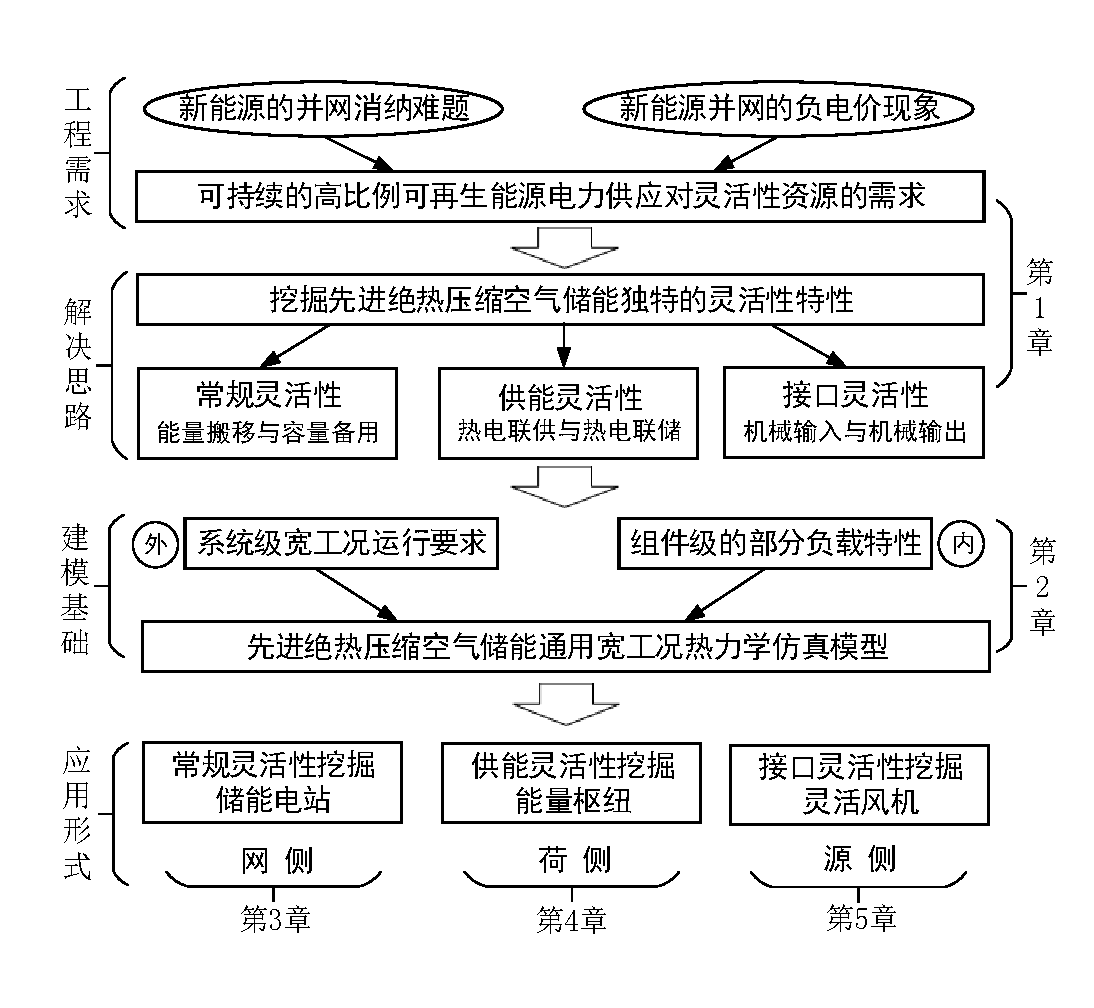
\includegraphics[scale=0.75]{figures/Chap1-4-Thesis-Framework-3.pdf}
  \caption{论文组织架构}
  \label{fig:Thesis-Framework}
\end{figure}

在\textbf{宽工况热力学特性仿真建模}方面,构建了计及组件部分负载运行特性的AA-CAES通用宽工况热力学仿真模型,并基于此分析了典型系统的运行性能。具体地:1)计及常压—常压、常压—滑压、滑压—常压、滑压—滑压等典型运行模式(压力视角),构建了基于热力学第一定律与热力学第二定律的仅电能供应与热电联供(温度视角)的通用稳态热力学仿真模型;2)采用构建的热力学仿真模型分析了典型AA-CAES系统在不同运行条件下的内部热力学特性及系统的整体供能特性,为网侧储能电站、荷侧能量枢纽及源侧风储集成等三种场景下对应AA-CAES应用形式的灵活性挖掘及运行模型的建立奠定基础。

在\textbf{挖掘以能量搬移与容量备用为特征的常规灵活性}方面,研究了以高效储能(灵活储能)形式支撑电力系统运行的AA-CAES 储能电站,并系统地提出了计及宽工况运行特性的储能电站建模、运行及运营方法。具体地:1)基于热力学宽工况仿真模型,提出了刻画AA-CAES独特的内部压力势能与压缩热能双能流解耦存储与耦合释能特性的宽工况热力学特性曲线簇;2)基于热力学特性曲线簇,构建了面向AA-CAES储能电站常规灵活性应用的宽工况储气—储热双SOC能量模型、能量与备用模型及其扩展模型;3)将双SOC 模型应用于风—储协同系统调度运行、日前电力市场策略竞标等问题,指导应用于电力系统的AA-CAES储能电站的建模、运行与运营。

在\textbf{挖掘以热电联供与热电联储为核心的供能灵活性}方面,研究了以能量枢纽(灵活负荷)形式支撑热电综合能源系统运行的AA-CAES型能量枢纽,并系统地提出了AA-CAES 型能量枢纽在热电综合能源系统的建模、运行及运营方法。具体地:1)设计了基于AA-CAES的两类热电联供能量枢纽,建立了表征其供能灵活性的热电联供模型;2)提出了集中式运营环境下含AA-CAES型能量枢纽的区域热电综合能源系统调度方法,并提出了基于㶲理论的热电综合能源系统数量—质量联合建模方法,为热电等多能流品位建模难题提供了新思路;3)提出了独立运营环境下面向热电综合能源市场的AA-CAES型能量枢纽的市场竞标策略,以实现能量枢纽的经济运行与运营。

在\textbf{挖掘以机械输入与机械输出为内涵的接口灵活性}方面,研究了以风-储集成系统(灵活电源)形式从源头平滑风电出力波动性的内嵌AA-CAES的可调度风机,并系统地提出了其建模、运行及运营等方法。具体地:1)设计了内嵌先进绝热压缩空气储能的灵活可调度风机,实现高风速时段叶片未利用风能的回收与低风速时段短缺风能的填补,从源头上降低了风速与风功率间的瞬时强耦合特性;2)提出了克服风速波动对内嵌AA-CAES运行效率影响的措施,建立了面向电力系统应用的灵活风机能量模型及双备用模型;3)在风机发电能力评估的基础上,提出了含灵活风机的电力系统调度运行及灵活风机市场竞标方法,以实现灵活风机的高效运行及运营。

本文通过分析面向新能源电力系统应用时AA-CAES内部组件的部分负载运行特性,建立了通用宽工况热力学仿真模型,从网侧高效储能电站、荷侧灵活能量枢纽、源侧灵活可调度风机三个角度系统研究了典型先进绝热压缩空气应用形式的设计建模、调度运行及市场运营等问题,为充分挖掘先进绝热压缩空气储能独特的储能循环的常规灵活性、供能灵活性及接口灵活性提供了较为系统的建模与分析方法,为实现可持续的高比例可再生能源电力供应提供了新的解决方案\footnote{尽管本文标题为源-网-荷先进绝热压缩空气储能灵活性建模及运行研究,但后续章节的实际组织则以网、荷、源的顺序开展,其主要原因在于:1)网侧储能电站利用的常规灵活性最直观,荷侧能量枢纽利用的供能灵活性也较易发现,而源侧风储集成系统利用的接口灵活性则不宜发觉,这也是我们在第\ref{sec:flexibility-intro}节先分析常规灵活性与供能灵活性,最后再分析接口灵活性的初衷;2)网侧储能电站、荷侧能量枢纽为电力系统注入的灵活性本质上是对新能源电力接入电力系统带来的不确定性及增加的灵活性资源需求的一种“被动补救”措施,而源侧风-储集成风机有望从源头上解决风电功率的波动性并降低对风电并网对系统灵活性资源的需求,可视为一种“主动预防”措施,按照“被动”-“主动”的逻辑组织结构更耐人寻味。}。总之,本文工作实现了一种“事后补救”与“提前预防”相结合的电力系统灵活性支撑方案,以网侧储能电站与荷侧能量枢纽“被动”满足当前电力系统的灵活性资源需求,提升现有电力系统对新能源的接纳能力;以源侧灵活风机在不增加(未来)风电的接入对系统灵活性资源的需求同时“主动”提供灵活性资源,从而满足未来电力系统对高比例新能源的并网消纳需求。

